\documentclass[11pt,a4paper]{article}
\usepackage[T1]{fontenc}
\usepackage[utf8]{inputenc}
\usepackage{lmodern,microtype}
\usepackage{amsmath,amssymb,amsthm,mathtools,bm}
\usepackage{booktabs,array,longtable}
\usepackage{graphicx,float,xcolor}
\usepackage[margin=2.05cm]{geometry}
\usepackage{enumitem,fancyhdr}
\usepackage[hidelinks,pdfencoding=auto]{hyperref}
\hypersetup{pdftitle={FIN ST327--ST341: Certified Coexistence, Mediator Rank, and Quantitative Observer Depth},pdfauthor={Krzysztof Żuchowski},pdfsubject={Analytical and interval continuation of FIN Release 10.78},pdfkeywords={FIN, information, localization, first-order transition, mediator, observer depth, Le Cam deficiency, holonomy, rate distortion, relative clocks}}
\definecolor{proved}{RGB}{20,92,48}\definecolor{conditional}{RGB}{148,88,0}\definecolor{blocked}{RGB}{150,28,28}
\newcommand{\Proven}{\textcolor{proved}{\textbf{[PROVEN]}}}\newcommand{\Evidence}{\textcolor{conditional}{\textbf{[STRONG NUMERICAL EVIDENCE]}}}\newcommand{\Partial}{\textcolor{conditional}{\textbf{[PARTIAL]}}}\newcommand{\Blocked}{\textcolor{blocked}{\textbf{[BLOCKED]}}}
\newtheorem{theorem}{Theorem}[section]
\pagestyle{fancy}\fancyhf{}\lhead{FIN ST327--ST341}\rhead{Release 10.79}\cfoot{\thepage}\setlength{\headheight}{14pt}\setlist[itemize]{leftmargin=1.3em,itemsep=2pt,topsep=3pt}\sloppy

\begin{document}\hypersetup{pageanchor=false}
\begin{titlepage}\centering
\vspace*{1cm}{\Large Fractal Information Theory Project\par}\vspace{.85cm}
{\huge\bfseries FIN ST327--ST341\par}\vspace{.35cm}
{\LARGE Certified Coexistence, Mediator Rank,\par}{\LARGE and Quantitative Observer Depth\par}
\vspace{.9cm}{\large Analytical, interval, and bounded computational research report\par}
\vfill{\Large Krzysztof \.{Z}uchowski\par}\vspace{.2cm}
{\large Independent Researcher --- Fractal Information Theory Project\par}{\large ORCID: 0009-0002-0909-3613\par}\vspace{.75cm}
{\large August 16, 2026\par}\vspace{.25cm}{\large Release 10.79\par}\vfill
\begin{minipage}{.92\textwidth}\small
\textbf{Repository snapshot.} Audited tracked base:
\texttt{bb540a767e210a5a3bf816e4868e7bcefbac3872}. The working tree contains uncommitted research artifacts; the release SHA-256 ledger identifies the files.

\medskip\textbf{License.} CC BY 4.0. \quad \textbf{Language.} English. \quad \textbf{Resource type.} Preprint and executable reproducibility package.
\end{minipage}\end{titlepage}
\hypersetup{pageanchor=true}\pagenumbering{roman}

\begin{abstract}
Programs ST327--ST341 continue the local mathematical program after Release 10.78. The
main advance is theorem-level local phase coexistence. Outward endpoint boxes and one
parametric Krawczyk tube prove a unique positive reflection-even stationary root for every
$g\in[2.900,2.905]$. Its objective is strictly positive at $g=2.900$ and strictly negative
at $g=2.905$, so at least one energy-equality crossing with the uniform state exists in that
interval. This is not yet a global transition: the exact 11-dimensional dual is compact on
the relevant sublevel, but a complete tensor cover exceeds the frozen budget by orders of
magnitude.

The localized branch has a well-conditioned augmented fold candidate at
$g\approx2.664908051$, still numerical. Lower-rank conservative mediators are classified
exactly: the optimal rank-$m$ Schur term retains the $m$ largest strict eigenmodes, with
Eckart--Young errors equal to the discarded spectral norms. A strict-invariant quartic
$\langle q,Aq\rangle^2$ supplies an admissible stabilizer shape, but its positive coefficient
is not sourced.

On the observer side, binary child-resolution instruments acquire an exact Le Cam depth:
for errors $e_f\le e_c<1/2$, the finer experiment has zero deficiency toward the coarser,
whereas reverse deficiency is $e_c-e_f$. Finite counts impose an $N^{-1/2}$ recovery floor.
Tree scale cocycles are gauge, but a cyclic refinement carries the gauge-invariant holonomy
$H=g_{01}g_{12}/g_{02}$. Approximate refinement preserves relative clocks within explicit
Weyl intervals. A declared correlated Markov branch process admits rate--distortion below
the arbitrary-history rate, showing precisely what fractal compression can mean after a
state class and loss function are supplied.

No strict source for active coupling or stabilizer coefficient, global physical vacuum,
selector closure, absolute unit, time arrow, Planck scale, spacetime, laboratory evidence,
legacy-role transfer, Standard Model, gravity, $L_{\rm total}$, or Theory-of-Everything
closure is claimed.
\end{abstract}
\tableofcontents\newpage\pagenumbering{arabic}

\section{Scope and proof discipline}

The strict object remains
\[
A=sI-W,\qquad W_{xx}=0,\qquad W_{xy}=K_{\rm strict}(d(x,y))\ (x\ne y),
\]
with $A\mathbf1=0$ and $A\succeq0$. The legacy kernel remains an intermediate bridge
object; no legacy role is transferred. The internal ontology remains informational
nadsoliton $\to$ light $\to$ matter $\to$ emergent observer, without a separate
informational layer below the nadsoliton. It is not used as a proof premise.

\Proven{} marks exact analysis or outward finite certification. \Evidence{} marks
reproducible floating computation. \Partial{} means a required continuous or global step
remains open. \Blocked{} records absent external evidence.

\section{Executive ledger}
\small
\begin{longtable}{p{.065\textwidth}p{.20\textwidth}p{.64\textwidth}}
\toprule Program&Status&Result\\\midrule\endhead
ST327&\Proven&A parametric root tube and opposite endpoint energy signs prove local coexistence crossing in $[2.900,2.905]$.\\
ST328&\Evidence&Simple-fold candidate at $g\approx2.664908051$; no 17-dimensional interval certificate.\\
ST329&\Proven{}+\Partial&Relevant dual sublevel is compact, but complete 11D tensor covering is outside the frozen budget.\\
ST330&\Proven&Exact optimal rank/error tradeoff for lower-rank conservative mediators.\\
ST331&\Proven{}+\Partial&Strict $A$ supplies a quartic invariant shape; its positive coefficient remains unsourced.\\
ST332&\Proven{}+\Partial&Projective observables have geometric tails; the weighted Chernoff derivative tail remains open.\\
ST333&\Partial&Only 26 of 40 isotropic overlapping slab attempts pass; continuous branch loss is not inferred.\\
ST334&\Proven{}+\Evidence&Finite multi-time IR design is an LP with dual threshold-band structure; grid solution is not a continuum theorem.\\
ST335&\Proven&Minimal cyclic refinement has gauge-invariant scale holonomy $H$.\\
ST336&\Proven&Exact Le Cam deficiency for binary partial child-resolution instruments.\\
ST337&\Proven&Finite-count scalar fiber recovery has an $N^{-1/2}$ minimax floor.\\
ST338&\Evidence&Block Markov rate--distortion demonstrates controlled correlated-history compression.\\
ST339&\Proven&Approximate intertwining yields explicit Weyl bounds for relative clock ratios.\\
ST340&\Proven&Dimensional rank and raw-$A$ unit incompatibility are separated from operational identifiability.\\
ST341&\Blocked&No independent raw-event packet exists.\\
\bottomrule\end{longtable}\normalsize

\section{ST327: a certified local coexistence transition}

For a reflection-even probability $p$ represented by seven orbit values $q_i$, stationarity
at supplied coupling $g$ is
\[
\log(12q_i)+1-g(Bq)_i+\lambda=0,
\qquad q_0+2\sum_{i=1}^{5}q_i+q_6=1.
\]
At $g=2.900$, the outward objective interval is
\[
[0.0016740014,\,0.0016751191],
\]
whereas at $g=2.905$ it is
\[
[-0.0016823923,\,-0.0016812705].
\]
Both endpoint roots lie in unique Krawczyk boxes. More importantly, one coordinatewise
parametric box contains a unique positive root for every $g$ in the complete interval; its
minimum inclusion margin is $6.7389\times10^{-5}$.

\begin{theorem}[certified local coexistence]
The positive reflection-even localized branch exists continuously throughout
$g\in[2.900,2.905]$ and has at least one point at which its objective equals that of the
uniform state.
\end{theorem}

This is the first theorem-level transition statement for the supplied negative-information
model. It is local coexistence, not a global phase transition: another state may have lower
energy, and the crossing need not be unique. The coefficient $g$ remains supplied.

\section{ST328--ST331: fold, globality, mediator rank, and stabilization}

The augmented equations
\[
F(x,g)=0,\qquad D_xF(x,g)v=0,\qquad \|v\|=1
\]
have a floating root at
\[
g_{\rm fold}\approx2.66490805100556.
\]
The residual is below $5\times10^{-14}$, the stationary Jacobian has one numerical null
direction, and the augmented Jacobian has minimum singular value about $0.255$. This is
strong evidence for a simple spinodal, but no outward 17-dimensional box was obtained.

ST329 proves a useful compactness result for the exact dual. On the mean-zero subspace,
\[
\frac1{2g}\langle h,A^+h\rangle-log\left(\frac1{12}\sum_i e^{h_i}\right)
\ge \frac{\|h\|^2}{2g\lambda_{\max}}-\|h\|.
\]
Hence every negative sublevel lies inside $\|h\|\le2g\lambda_{\max}\approx18.7375$.
The problem is compact, but a mere $16$-cell partition per axis already contains
$16^{11}=17{,}592{,}186{,}044{,}416$ boxes. The frozen million-box budget cannot support a
tensor cover. This is a method no-go, not a globality verdict.

For a mediator of dimension $m$, the induced Schur matrix has rank at most $m$.
\begin{theorem}[optimal lower-rank mediator]
Among positive semidefinite matrices of rank at most $m$, the best approximation to $gA$
in either Frobenius or operator norm retains the $m$ largest eigenvalues and modes of $gA$.
The errors are respectively
\[
\left(\sum_{j>m}\sigma_j^2\right)^{1/2},\qquad \sigma_{m+1}.
\]
\end{theorem}

\begin{figure}[H]\centering
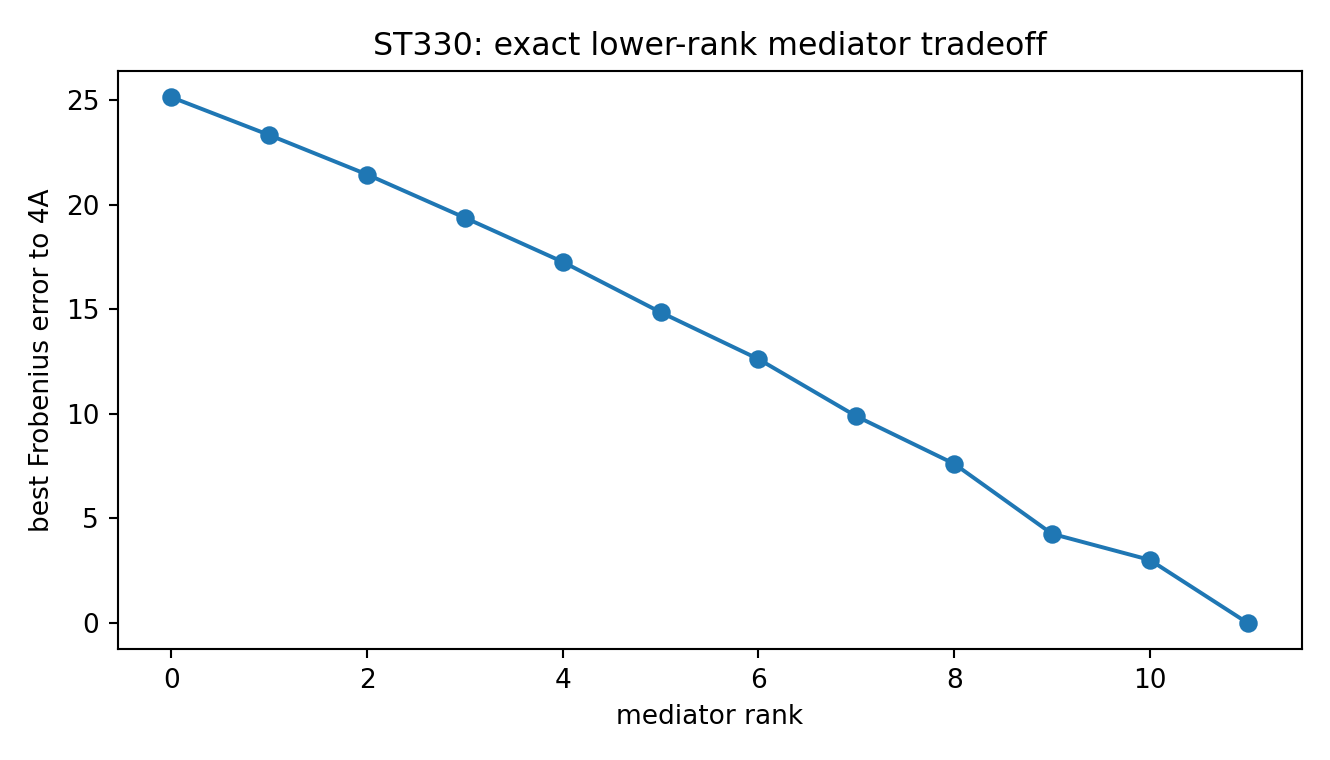
\includegraphics[width=.75\textwidth]{FIN_ST327_ST341_Figures/st330_rank_tradeoff.png}
\caption{Exact cost of reducing the conservative mediator below the full rank 11 required for $gA$.}
\end{figure}

Lower-rank mediation therefore selects stiff modes rather than reproducing the full strict
geometry. FIN currently supplies no rule selecting the rank or coupling.

An admissible stabilizer is
\[
V_{g,c}(p)=D(p\|u)-\frac g2Q+\frac c4Q^2,
\qquad Q=\langle p-u,A(p-u)\rangle.
\]
The shape is $D_{12}$-invariant and constructed only from strict $A$; $c>0$ stabilizes an
unconstrained mean-zero carrier. But the probability simplex is already compact, and $A$
does not choose the coefficient or its sign. This is a completion template, not a sourced
law.

\section{ST332--ST334: tails, branch tubes, and multi-time infrared design}

The exact filter contraction $\rho=5/7$ implies that every projective-Lipschitz observable
with constant $L$ has future dependence tail at most
\[
\frac{L\rho^n}{1-\rho}.
\]
For the frozen one-step log-weight oscillation $L\le\log49$, this drops from about $1.29$ at
depth 7 to $2.78\times10^{-11}$ at depth 80. The full Chernoff derivative also differentiates
multiplicative weights; no uniform normalized derivative Lipschitz constant was certified.
Belief forgetting is proved, optimizer promotion is not.

ST333 tests 40 wider isotropic boxes intended to overlap the ST298 sections. Twenty-six pass
and fourteen fail. The first failures are recorded in the packet. This falsifies that simple
enclosure strategy, not the existence of the branch. A true parameterized tube needs
separate longitudinal and transverse widths.

For several observer times $t_j$, the soft-IR problem is the linear program
\[
\max_{0\le q\le1}z,quad \int d_{t_j}(\mu)q(\mu)d\log\mu\ge z,quad
\int h(\mu)q(\mu)d\log\mu\le B.
\]
LP duality proves a threshold rule for one weighted combination of the active time kernels
minus the heat price. Unlike the single-time bathtub order, several bands can occur. The
500-point, three-time grid gives minimax value $1.2763170$ under budget $3$, but remains a
finite discretization.

\section{ST335--ST337: cyclic calibration and quantitative observer depth}

Tree cocycles are gauge-trivial. The smallest nontrivial refinement diagram is a triangle.
Under vertex calibration changes, the edge rates change but
\[
H=\frac{g_{01}g_{12}}{g_{02}}
\]
does not. $H=1$ is path independence; $H\ne1$ is relative calibration curvature. This is a
complete one-cycle classification, but FIN has not supplied a physical cyclic refinement
or a value of $H$.

The qualitative Blackwell order can be made quantitative. Let a child-resolving instrument
be a binary symmetric channel with error $e$.
\begin{theorem}[exact binary observer depth]
For $0\le e_f\le e_c<1/2$,
\[
\delta(\mathrm{BSC}(e_f),\mathrm{BSC}(e_c))=0,
\qquad
\delta(\mathrm{BSC}(e_c),\mathrm{BSC}(e_f))=e_c-e_f.
\]
\end{theorem}
The finer instrument simulates the coarser by adding noise. The reverse direction cannot
increase total-variation separation. This creates a continuous operational layer depth
between exact resolution and blindness. It is an instrument theorem, not a theory of
consciousness or proof of a physical FIN layer.

Ideal identifiability also does not remove sampling cost. Le Cam's two-point method gives a
scalar child-probability minimax floor of order $N^{-1/2}$. Extending to 78 free symmetric
fiber parameters requires at least order $78/\epsilon^2$ effective independent counts before
confidence and conditioning factors. No local code can replace those events.

\section{ST338--ST340: controlled compression, approximate clocks, and dimensions}

ST326 proved that arbitrary binary branch histories require one bit per layer. Compression
becomes possible only after defining a state class. ST338 chooses a stationary binary
Markov class with flip probability $0.1$ and normalized Hamming distortion. Its asymptotic
lossless entropy rate is
\[
h_2(0.1)\approx0.468996\ \text{bits per layer},
\]
already below the arbitrary-history rate. An eight-layer Blahut--Arimoto computation gives
the displayed finite-block rate--distortion curve.

\begin{figure}[H]\centering
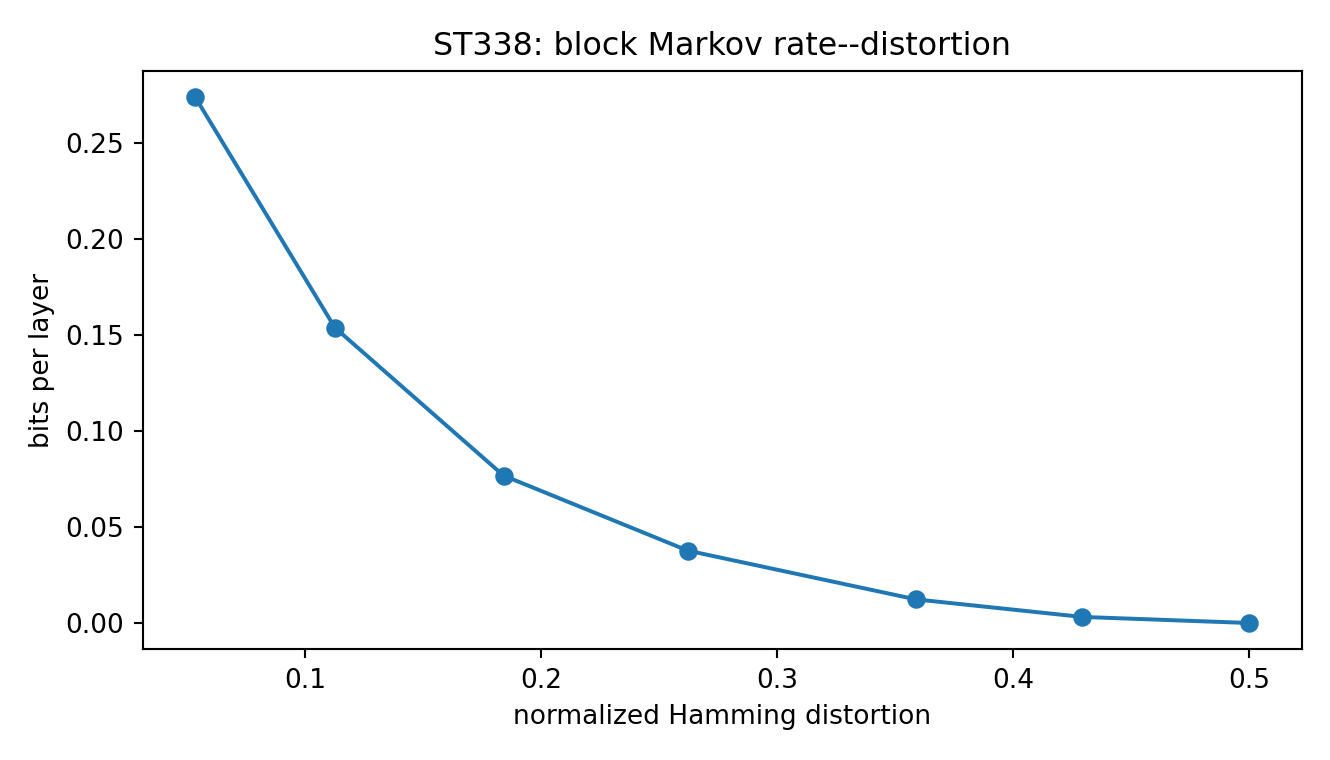
\includegraphics[width=.73\textwidth]{FIN_ST327_ST341_Figures/st338_rate_distortion.png}
\caption{Controlled compression after supplying a correlated source class and a distortion measure.}
\end{figure}

This is the rigorous form of the useful fractal-compression intuition: a short rule plus
correlations and allowed distortion can reduce record cost. The Markov law, its parameter,
and the distortion are not derived from FIN.

Relative clocks are stable when exact intertwining is weakened. If the compressed refined
operator differs from $A$ by operator norm at most $\epsilon<\lambda_1$, Weyl's theorem gives
\[
\frac{\lambda_j-\epsilon}{\lambda_i+\epsilon}
\le\frac{\widetilde\lambda_j}{\widetilde\lambda_i}
\le\frac{\lambda_j+\epsilon}{\lambda_i-\epsilon}.
\]
Wave-clock ratios obey the square roots of these bounds. This controls relative drift; it
does not produce seconds or a time arrow.

Finally, dimensional relations and channel identification are separate obligations. In
basis $(L,T,E)$, a speed row $(1,-1,0)$ and action row $(0,1,1)$ have rank two. Adding an
independent diffusion row can reach rank three. Repeating $ET$ does not. More basically,
one raw $A$ cannot simultaneously carry dimension $T^{-1}$ for unitary/heat evolution and
$T^{-2}$ for wave evolution. Distinct sector conversion maps are necessary and must be
operationally calibrated.

\section{Falsification ledger and current interpretation}
\begin{longtable}{p{.27\textwidth}p{.29\textwidth}p{.37\textwidth}}
\toprule Claim&Test&Surviving statement\\\midrule\endhead
The sampled crossing was enough&Parametric root tube and interval energies&Now repaired: at least one local crossing in $[2.900,2.905]$ is proved.\\
The crossing is a global transition&Compact dual plus cover audit&Still unproved; naive 11D tensor certification is infeasible under the frozen budget.\\
The spinodal is proved&Augmented fold system&Only strong numerical evidence at $g\approx2.664908051$.\\
Small mediator reproduces strict gain&Eckart--Young classification&False exactly below rank 11; lower ranks approximate selected stiff modes.\\
Strict symmetry supplies stabilization completely&Quartic invariant audit&It supplies a shape, not a positive coefficient.\\
Belief contraction closes Chernoff asymptotics&Weighted derivative audit&False so far; weight derivatives require another uniform constant.\\
All scale cocycles are gauge&Minimal cycle&False on cyclic diagrams; holonomy is gauge invariant.\\
Observer depth is merely qualitative&Binary deficiency theorem&False in the declared family; exact quantitative depth is $e_c-e_f$.\\
Fractal compression is impossible&Markov rate--distortion&False for restricted correlated sources; arbitrary-history lower bounds remain intact.\\
Relative clocks collapse under small error&Weyl bounds&False; they vary continuously inside explicit intervals.\\
Local work supplies evidence&Independent-record gate&False; ST341 remains blocked.\\
\bottomrule\end{longtable}

The deepest surviving interpretation is:
\begin{quote}
With a supplied signed interaction, FIN now possesses a theorem-level localized branch and
a certified local coexistence crossing. What remains missing is global variational closure
and a strict source for the coupling and stabilization coefficient. Refinement supports a
quantitative hierarchy of accessible information, gauge-invariant calibration holonomy on
cycles, and robust relative clocks. Fractal compression is meaningful only relative to a
source class and tolerated distortion. These are precise mathematical bridges, but none
selects SI units, an apparatus, or our observed universe without additional operational and
empirical structure.
\end{quote}

\section{Recommended programs ST342--ST356}
\begin{enumerate}
\item[\textbf{ST342}.] Narrow the certified coexistence bracket using interval bisection on the parametric root tube.
\item[\textbf{ST343}.] Build a full 17-dimensional interval Krawczyk certificate for the fold candidate.
\item[\textbf{ST344}.] Reduce the exact global dual by $D_{12}$ orbit types and derive a symmetry-safe lower envelope before any branch-and-bound.
\item[\textbf{ST345}.] Prove or refute that every global minimizer at $g=4$ is reflection-equivalent to the certified localized orbit.
\item[\textbf{ST346}.] Couple optimal rank-$m$ mediators to the simplex and determine which modal truncation first produces localization.
\item[\textbf{ST347}.] Classify all degree-four and degree-six strict invariants that can stabilize the carrier and expose every free coefficient.
\item[\textbf{ST348}.] Derive the missing normalized Chernoff derivative Lipschitz constant or construct a counterexample.
\item[\textbf{ST349}.] Replace isotropic branch boxes by anisotropic interval implicit-function slabs.
\item[\textbf{ST350}.] Certify the continuum multi-time IR dual with finitely supported dual measures or prove that support must grow.
\item[\textbf{ST351}.] Classify scale holonomy on two-cycle refinement complexes and its independent cohomology rank.
\item[\textbf{ST352}.] Extend Le Cam observer depth from BSC instruments to the 12-child circulant confusion family.
\item[\textbf{ST353}.] Derive sharp finite-count lower and upper bounds for recovering a spectrally restricted fiber $B$.
\item[\textbf{ST354}.] Estimate rate--distortion for a source law generated by a declared FIN transition kernel, keeping the law explicitly conditional.
\item[\textbf{ST355}.] Propagate approximate-clock bounds through multiple refinement levels and separate accumulated drift from gauge calibration.
\item[\textbf{ST356}.] Resume empirical analysis only after independently registered, hashed raw events and separated custody roles exist.
\end{enumerate}

The highest priorities are ST343 and ST344: they target the remaining local fold certificate
and the global variational obstruction. ST352 is the strongest continuation of the internal
observer program because it moves from a binary toy family to the actual 12-state symmetry
without claiming an apparatus.

\section{Reproducibility and conclusion}

The executable source \texttt{fin\_st327\_st341\_research.py} writes fifteen packets, an
aggregate JSON, a CSV ledger, and two figures. The independent suite
\texttt{test\_fin\_st327\_st341.py} performs sixteen live checks of packet hashes, crossing
signs, parametric inclusion, the fold residual, cover-budget stop, mediator error monotonicity,
stabilizer status, projective tails, slab failure, LP feasibility, holonomy invariance,
deficiency, finite-count scaling, rate--distortion monotonicity, Weyl containment,
dimensional rank, and the evidence stop. All sixteen tests pass.

Release 10.79 closes one important gap: local coexistence is now a theorem rather than a
plot. It also shows why this is not yet physical closure. Globality, signed-source origin,
stabilization strength, dimensional calibration, apparatus, and independent events remain
separate obligations. The observer and compression ideas survive in more rigorous forms:
deficiency rather than pictorial depth, holonomy rather than arbitrary scale rate, and
rate--distortion rather than cost-free storage of arbitrary histories.

\end{document}
